% Compile with: pdflatex (run TWICE to resolve cross-references), or paste into Overleaf.
\documentclass[11pt]{article}
\usepackage[letterpaper, margin=1in, top=0.8in, bottom=0.8in]{geometry}
\usepackage[T1]{fontenc}
\usepackage[utf8]{inputenc}
\usepackage{palatino}
\usepackage{microtype}
\usepackage[htt]{hyphenat}
\usepackage{amsmath}
\usepackage{amssymb}
\usepackage{titlesec}
\usepackage{enumitem}
\usepackage{booktabs}
\usepackage{float}
\usepackage{graphicx}
\usepackage{caption}
\usepackage{hyperref}
\captionsetup{font=small, skip=4pt}

\titleformat{\section}{\normalfont\normalsize\bfseries}{\thesection.}{0.5em}{}
\titlespacing*{\section}{0pt}{1em}{0.3em}

\setlength{\parskip}{0.5em}
\setlength{\parindent}{0pt}
\setlength{\emergencystretch}{3em}
\setlist{itemsep=0.15em, topsep=0.2em, partopsep=0pt, leftmargin=1.4em}

\begin{document}

\begin{center}
  {\large\bfseries Epic Games Store Giveaways: Causal Effect on Steam Player Engagement}\\[0.4em]
  {\small Nicholas Liu \quad|\quad 14.33 --- Descriptive Table and Figure}
\end{center}

\vspace{0.5em}
\hrule
\vspace{0.8em}

\section{Overview}

This project studies whether free game giveaways on the Epic Games Store (EGS) causally
increase player engagement on Steam for the same title. The key outcome variable is the
monthly average number of concurrent Steam players (log-transformed). I use a staggered
difference-in-differences event study, exploiting variation in the timing of each game's
first Epic giveaway as the treatment.

\section{Data Structure and Sample Restrictions}

\textbf{Unit of observation.} The analysis uses a game--month panel. Each observation
records a single game's SteamCharts-reported average and peak concurrent player count for
one calendar month.

\textbf{Panel dimensions.} The assembled panel spans \textbf{July 2012 through
February 2026} (164 calendar months) and contains \textbf{38,642 game--month
observations} across \textbf{446 unique games}. Coverage is unbalanced: each game's
time series begins near its Steam release date and ends at the scrape cutoff, so
observation lengths differ substantially across titles. The median game contributes
\textbf{88 months} of data; 27 games have fewer than 24 months and 12 have fewer
than 12 months.

\textbf{Sample restrictions applied before analysis:}
\begin{itemize}
  \item \textit{Unmatched Epic titles.} Eight Epic giveaway titles confirmed absent from
    Steam (five EGS exclusives and three placeholder entries in the Kaggle source) are
    excluded from the panel entirely.
  \item \textit{Missing SteamCharts data.} Thirteen games returned HTTP 500 errors
    during scraping and have no player-count data; they are excluded.
  \item \textit{Duplicate App ID collisions.} Four cases where two distinct Epic game
    names resolved to the same Steam App ID are collapsed to a single panel entry,
    retaining the earliest giveaway date as the treatment.
\end{itemize}

\textbf{Treatment variable.} All 446 games in the panel are eventually treated (Epic
giveaways were the source criterion for inclusion). Treatment is defined as the calendar
month of each game's \textit{first} Epic free giveaway. Of the 446 treated games, 421 have SteamCharts data covering the treatment month, and
336 have a full $[-12,+12]$ event window for the event-study regression.
Treatment cohorts are distributed across 80 distinct calendar months, with the bulk
concentrated in 2019--2023.

\textbf{Outcome variable.} The regression outcome is $\ln(\texttt{avg\_players}+1)$,
where $\texttt{avg\_players}$ is the SteamCharts monthly average concurrent player count
(in raw players). The $+1$ offset handles months with zero reported players (common for
low-traffic titles) and the log transformation compresses the heavy right tail driven by
a small number of AAA titles.

\section{Summary Statistics}

Table~\ref{tab:sumstats} presents summary statistics for the key variables. All
game--month rows use $N = 38{,}642$ observations; the final row (\textit{months observed
per game}) is at the game level ($N = 446$).

The raw player counts are highly right-skewed: the mean monthly average of
$1{,}584$ players is more than 24 times the median of $65$ players, and the maximum
of $270{,}553$ reflects large-player-base titles such as GTA V and Destiny~2. The
log-transformed outcome is far better behaved (mean 4.43, SD 2.36), as intended. The
repeat-event indicator equals 1 in months within 12 months after a game's
\textit{second or later} Epic giveaway; only 2\% of game--month observations have this
flag, since most games were given away exactly once.

\begin{table}[h]
\centering\small
\caption{Summary statistics --- Epic giveaway panel}
\label{tab:sumstats}
\begin{tabular}{lrccccc}
\toprule
Variable & $N$ & Mean & SD & Min & Median & Max \\
\midrule
Avg.\ concurrent Steam players (monthly) & 38,642 & 1,583.9 & 7,444.0 & 0.00 & 65.2 & 270,553 \\
Peak concurrent Steam players (monthly)  & 38,642 & 3,214.1 & 14,861.2 & 0 & 171 & 527,652 \\
$\ln(\texttt{avg\_players}+1)$ [outcome] & 38,642 & 4.43 & 2.36 & 0.00 & 4.19 & 12.51 \\
Repeat-giveaway window indicator (0/1)   & 38,642 & 0.02 & 0.15 & 0 & 0 & 1 \\
\midrule
Months of SteamCharts data per game & 446 & 86.6 & 41.1 & 1 & 88 & 163 \\
\bottomrule
\end{tabular}
\medskip

\noindent\small\textit{Notes:} Game--month panel, 446 games, July 2012--February 2026.
  Player counts are in \textit{raw players} as reported by SteamCharts.com.
  The outcome variable $\ln(\texttt{avg\_players}+1)$ uses a +1 offset to accommodate
  months with zero reported players.
  The repeat-giveaway window indicator equals 1 in months falling within 12 months
  after a game's second (or later) Epic giveaway.
  The bottom row is game-level ($N = 446$ unique games).
\end{table}

\section{Figures}

\subsection*{Figure 1: Outcome Variable Distribution and Unconditional Event-Time Profile}

Figure~\ref{fig:outcome} presents two panels. The \textbf{left panel} shows overlaid
density histograms of the log-transformed outcome variable for pre-giveaway months
($k < 0$, i.e., months before the first Epic giveaway) and post-giveaway months
($k \geq 0$). The distributions are broadly similar in shape---both are roughly
unimodal with a long right tail---but the post-giveaway distribution is shifted
left: the mean of the post distribution is lower than that of the pre distribution
by approximately 0.28 log points (roughly 25\% in levels). This unconditional
comparison is confounded by composition: post-giveaway months pool across many
games and calendar years, including more low-traffic titles. The large mass near
zero in both distributions reflects the 123 games with fewer than 10 median
monthly concurrent players; these near-zero-count games dominate the lower tail
when log-transformed.

The \textbf{right panel} plots the unconditional mean of the outcome variable at
each event-time $k \in [-12, 12]$, with 95\% confidence intervals computed across
all games observed at that relative period. This is a raw analog of the event-study plot: it does \textit{not} control for game
or calendar-time fixed effects, so level differences partly reflect cohort
composition and life-cycle stage. Nonetheless, two features of
the raw profile are notable. First, the pre-period mean is approximately flat across
$k \in [-12, -1]$, providing preliminary (unconditional) support for the parallel
trends assumption. Second, there is a sharp visible uptick at $k = 0$ (the giveaway
month itself), consistent with a positive contemporaneous treatment effect that is
subsequently partially sustained in months $k = 1$ through $k = 12$.

\subsection*{Figure 2: Panel Descriptives --- Pre-Treatment Distribution, Cohort Timing, and Repeat Structure}

Figure~\ref{fig:desc} provides three additional panels characterizing the panel's
structure.

\textbf{Panel (a): Pre-treatment player distribution.} The log-transformed
pre-treatment median player count across 446 games is right-skewed, with many
low-traffic titles and a long tail of more popular ones, motivating the
popularity-stratified robustness checks in the main analysis.

\textbf{Panel (b): Treatment cohort by year.} First-giveaway cohorts are broadly
evenly distributed across 2019--2023. The 2018 cohort is small (program launched
December 2018); 2024--2025 cohorts are smaller due to truncation at the February
2026 scrape. This spread provides the timing variation for staggered DiD.

\textbf{Panel (c): Repeat-giveaway share.} The fraction of games with a proximate
repeat giveaway (second event within 12 months of the first) ranges from 0\% to about
20\% across cohort years, averaging roughly 10\%. These roughly 30 games are the
primary source of identifying variation for the repeat-event coefficient $\hat{\delta}$.

\begin{figure}[H]
\centering
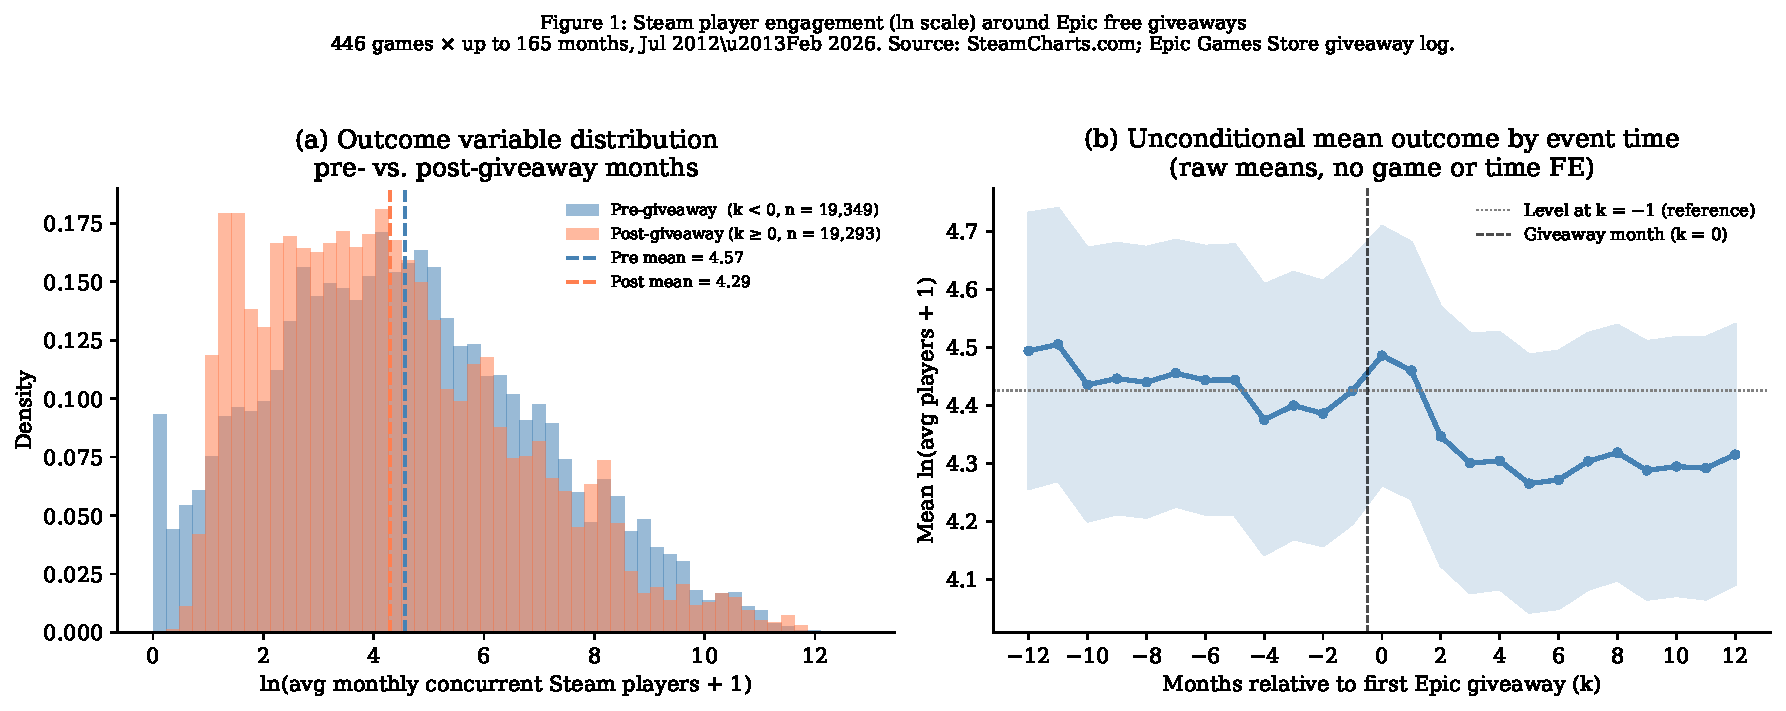
\includegraphics[width=0.88\linewidth]{../output/fig_outcome_histogram.pdf}
\caption{Steam player engagement (log scale) around Epic free giveaways.
  \textbf{Left:} Density histogram of $\ln(\texttt{avg\_players}+1)$ for pre-giveaway
  months ($k < 0$, blue) and post-giveaway months ($k \geq 0$, orange), pooled across all 446 games.
  \textbf{Right:} Unconditional mean (with 95\% CI) of the outcome by event-time $k \in [-12,12]$;
  the dashed vertical line marks the giveaway month ($k = 0$). Both panels use 38,642
  game--month observations.
  \textit{Source:} SteamCharts.com; Epic Games Store giveaway log (Kaggle, Dongre 2025).}
\label{fig:outcome}
\end{figure}

\begin{figure}[H]
\centering
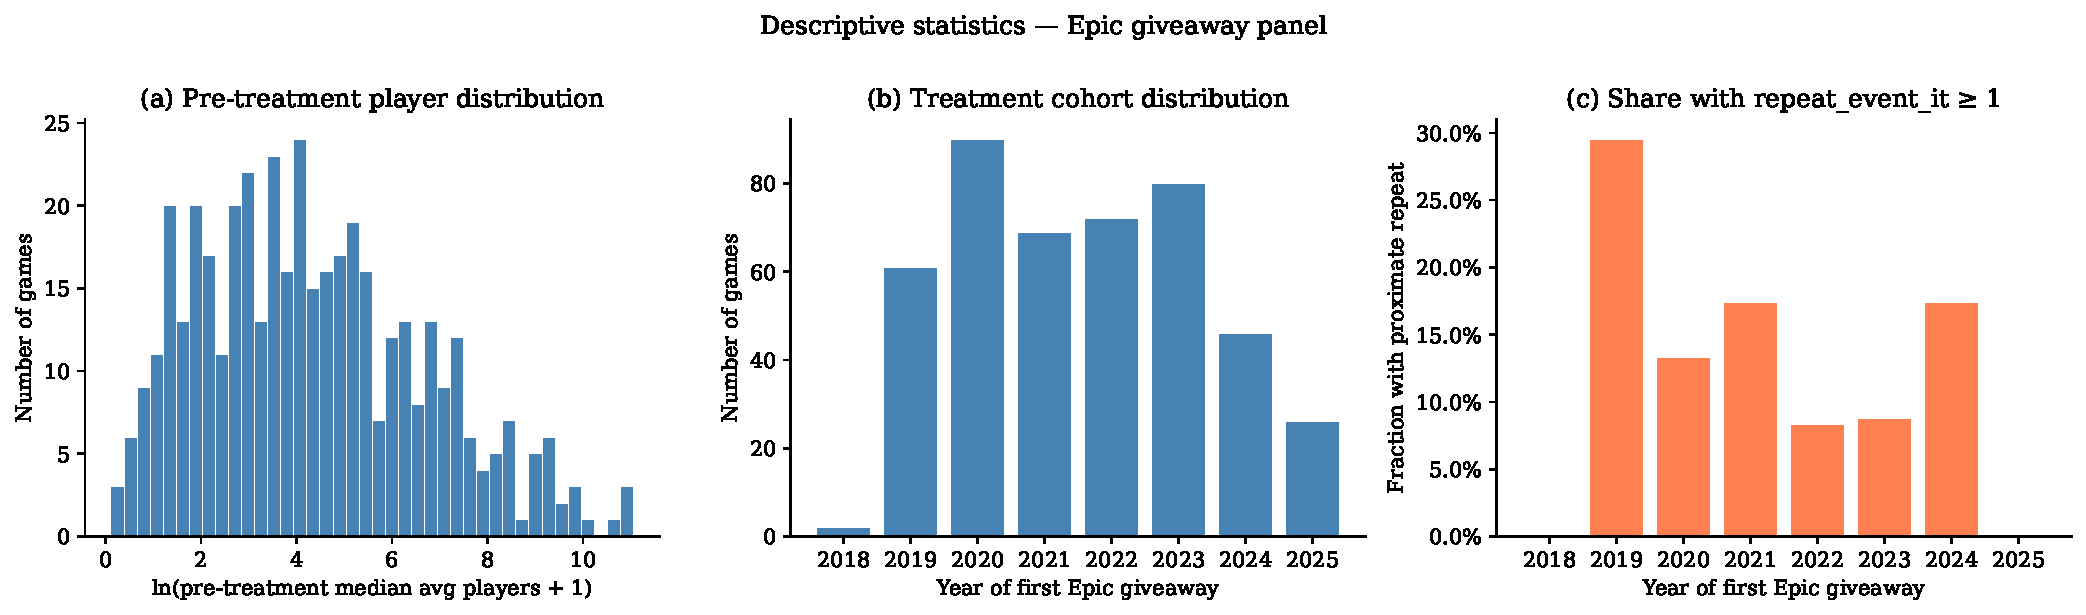
\includegraphics[width=0.88\linewidth]{../output/fig_descriptives.pdf}
\caption{Panel structure and descriptive statistics.
  \textbf{(a)} Histogram of $\ln(\text{pre-treatment median avg players} + 1)$ across 446
  games, illustrating heterogeneity in baseline Steam popularity.
  \textbf{(b)} Number of games with first Epic giveaway in each calendar year (2018--2025).
  \textbf{(c)} Fraction of games with a proximate repeat giveaway
  (second giveaway within 12 months of first) by cohort year.
  \textit{Source:} SteamCharts.com; Epic Games Store giveaway log (Kaggle, Dongre 2025).}
\label{fig:desc}
\end{figure}

\vspace{1.5em}
\noindent\rule{\textwidth}{0.4pt}
\vspace{0.3em}

\noindent\textit{Note on AI usage: I used AI to assist with drafting and formatting this document in \LaTeX.}

\end{document}
